\documentclass[journal,twoside,web]{ieeecolor}
\pdfobjcompresslevel=0   % disable object-stream compression (avoids the buffer overflow)
\pdfcompresslevel=9      % compress streams (keeps file size reasonable)
\pdfminorversion=5       % optional: lower PDF version compatibility if needed

\usepackage{jsen}
\usepackage{cite}
\usepackage{amsmath,amssymb,amsfonts}
%\usepackage{algorithmic}
\usepackage{graphicx}
\usepackage{caption}
\usepackage{subcaption}
\usepackage{textcomp}
\usepackage{float}
\usepackage{wrapfig}
\usepackage{tabularx}
\usepackage{multirow}
\usepackage{siunitx}  % For S columns and \sisetup
\usepackage{booktabs} % For \toprule, \midrule, \bottomrule
\usepackage[table]{xcolor}  % For \rowcolor (this also loads colortbl)
\usepackage{multirow}
\usepackage[english]{babel}
\usepackage[utf8]{inputenc}
\usepackage{algorithm}
\usepackage{comment}
%\usepackage{algorithm2e}
\usepackage{algorithmic}
\usepackage{algorithm}
\usepackage{pifont}
\usepackage{hyperref}
\usepackage{makecell}

%\pgfplotsset{compat=1.18}

\pdfobjcompresslevel=0
\pdfminorversion=5

\newcommand{\cmark}{\ding{51}}%
\newcommand{\xmark}{\ding{55}}%

%\usepackage{algpseudocode}
\def\BibTeX{{\rm B\kern-.05em{\sc i\kern-.025em b}\kern-.08em
    T\kern-.1667em\lower.7ex\hbox{E}\kern-.125emX}}
\markboth{\journalname, }
{Author \MakeLowercase{\textit{et al.}}: Preparation of Papers for IEEE TRANSACTIONS and JOURNALS (February 2017)}
\definecolor{abstractbg}{rgb}{0.89804,0.94510,0.83137}
\setlength{\fboxrule}{0pt}
\setlength{\fboxsep}{0pt}
\begin{document}
\title{TMCR Edge-YOLO: Thermal Sensing-based Mobility-Context Recognition on the Edge}
\begin{comment}
\author{Bethi Pardhasaradhi, \IEEEmembership{Member, IEEE}, and Linga Reddy Cenkeramaddi, \IEEEmembership{Member, IEEE}
\end{comment}
\author{Advik Manda, Bethi Pardhasaradhi, %\IEEEmembership{Member, IEEE} 
and Linga Reddy Cenkeramaddi, \IEEEmembership{Senior Member, IEEE}
\thanks{Compiled on \today. 
}
\thanks{Bethi Pardhasaradhi, and Linga Reddy Cenkeramaddi are with the autonomous and cyber-physical systems (ACPS) research group, Department of Information and Communication Technology (ICT), University of Agder, Campus Grimstad, Jon Lilletuns Vei 9, 4879, Grimstad, Norway (e-mail: pardhasaradhi.bethi@uia.no, linga.cenkeramaddi@uia.no.) }
\thanks{Advik Manda is with Department of Electronics and Communications Engineering (ECE), Indian Institute of Information Technology, Design and Manufacturing (IIITDM), Kancheepuram, 600127, India. and with the autonomous and cyber-physical systems (ACPS) research group, Department of Information and Communication Technology (ICT), University of Agder, Campus Grimstad, Jon Lilletuns Vei 9, 4879, Grimstad, Norway (e-mail: advik2040@gmail.com.)}
}

\IEEEtitleabstractindextext{%
\fcolorbox{abstractbg}{abstractbg}{%
\begin{minipage}{\textwidth}%
\begin{wrapfigure}[14]{r}{3in}%
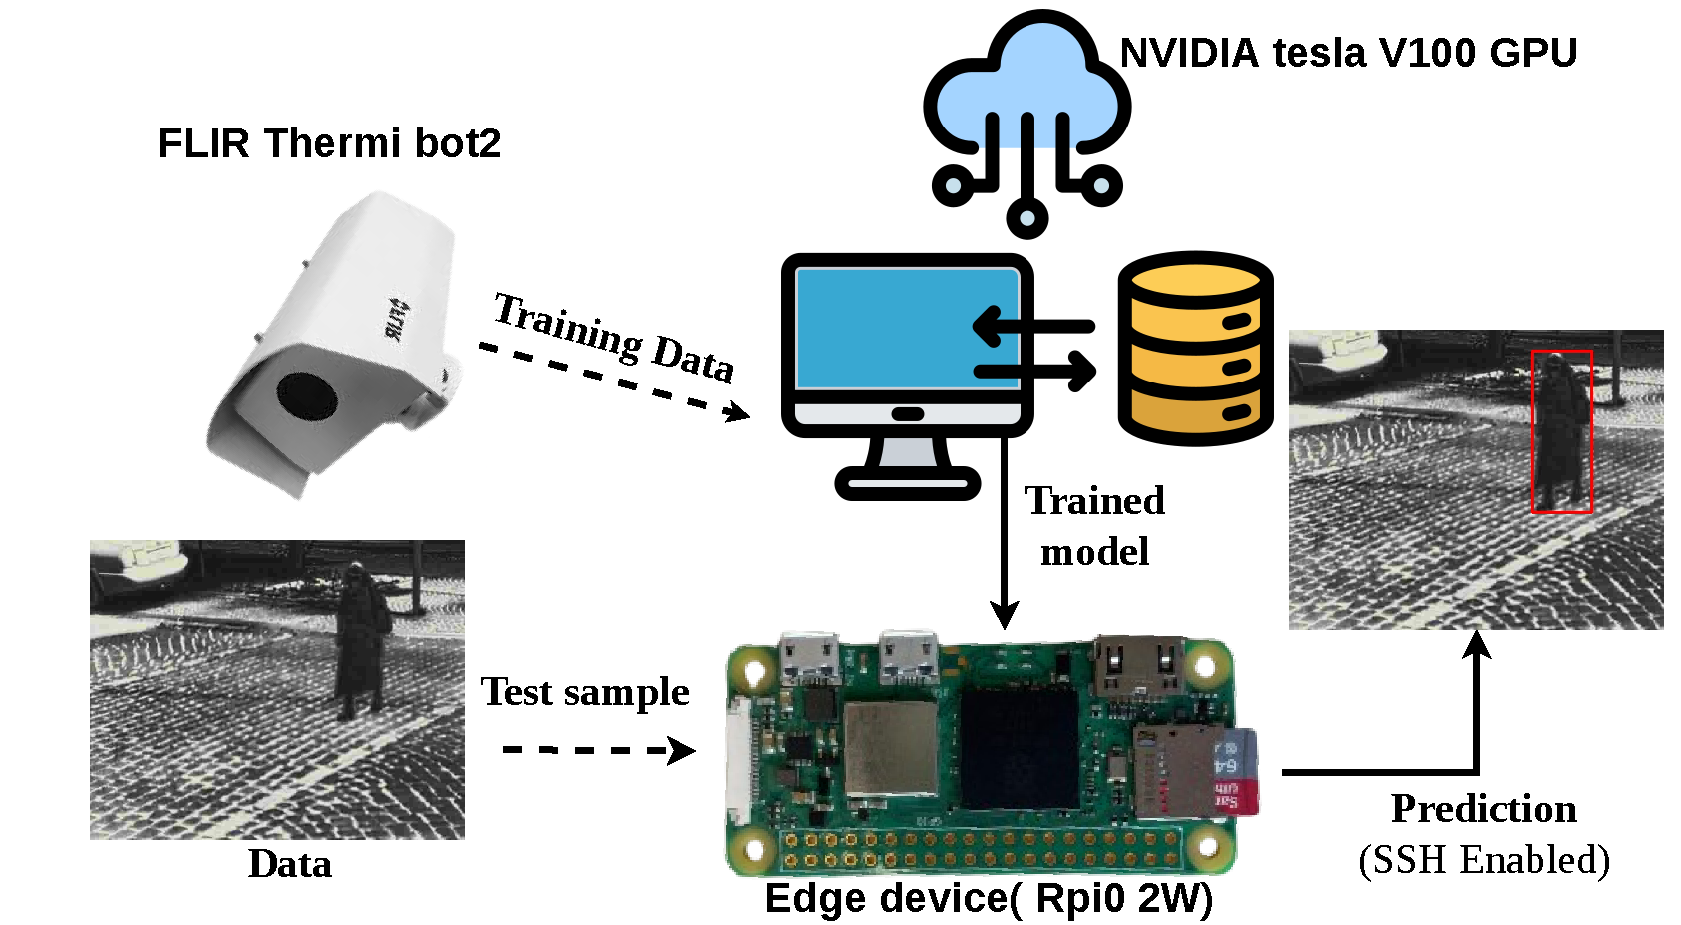
\includegraphics[width=2.9in]{yolo_thermal_front.pdf}%
\end{wrapfigure}%
\begin{abstract}
Thermal infrared (IR) sensors provide illumination-invariant perception and privacy-preserving monitoring for smart environments, assistive mobility, and human-centric analytics. However, existing IR detection systems typically treat pedestrians as a single class and do not capture the diversity of mobility contexts encountered in real settings, where individuals may use assistive devices, carry loads, or interact with dependent/personal transport objects. This creates a coupled sensing challenge: recognizing fine-grained mobility-context signatures in low-contrast thermal imagery while maintaining deployment feasibility on resource-constrained edge platforms. This work introduces the Thermal Mobility Context Recognition (TMCR) problem, which focuses on identifying distinct mobility signatures in thermal imagery that describe how people move and interact with their surroundings. Data were acquired using FLIR ThermiBot~2 cameras across twelve categories, including walking, wheelchairs, rollators, crutches, blind sticks, walking sticks, strollers, bicycles, luggage, shopping trolleys, and dogs. These classes are organized into five semantic groups: general agents, wheeled mobility assistance, non-wheeled mobility assistance, load-bearing objects, and personal or dependent transport. To jointly address thermal discriminability and edge efficiency, we develop a lightweight dual-attention YOLO-Thermal architecture that is co-optimized for IR imaging and embedded inference. A key contribution of this work is a cloud-edge methodology in which all training, annotation, and model optimization are performed in the cloud, while inference is executed entirely on the edge. This separation enables high-compute learning in the cloud and low-latency prediction on compact thermal sensing nodes. The proposed model achieves an mAP\(_{50\text{--}95}\) of 89.9\%, which is 3.37\% higher than YOLOv8s, while using only 4.9 million parameters. Cross-platform evaluation demonstrates edge-feasible deployment on edge platforms such as Raspberry~Pi~Zero 2W, Raspberry~Pi~5, NVIDIA Jetson AGX Xavier, and Rock Pi 4 C+ boards. The inference latency is \textbf{6183.36\,ms on Pi Zero} and \textbf{726.28\,ms on Pi 5}. These results show that the contribution is not only a thermal dataset, but a combined sensing--modeling--deployment framework in which cloud-trained and edge-executed thermal models enable context-aware mobility understanding for privacy-preserving intelligent sensing applications.

\end{abstract}


\begin{IEEEkeywords}
	Infrared Object Detection, YOLO, Attention Mechanisms, Dual Attention, Channel Attention, Spatial Attention, Lightweight Object Detection, Optimized Residual Block, Custom Architecture.
\end{IEEEkeywords}
\end{minipage}}}
\maketitle
\section{Introduction}
Infrared (IR) and thermal imaging sensors have become fundamental components of modern perception systems, enabling robust human detection and environmental awareness under poor lighting and adverse weather conditions~\cite{wilson2023recent}. Unlike visible-light cameras, thermal sensors operate independently of ambient illumination and inherently preserve privacy by capturing temperature-dependent information rather than identifiable textures. These properties make them suitable for intelligent transportation~\cite{zhang2020traffic}, assistive mobility~\cite{breland2021robust}, and smart-city monitoring applications~\cite{guan2018daily}. The integration of thermal sensing with embedded AI has further enabled intelligent edge nodes capable of local decision-making and event recognition without continuous cloud connectivity, thereby reducing latency, communication overhead, and energy consumption.

Thermal imaging is applied in diverse domains, including activity recognition%~\cite{min2025human}
, transportation%~\cite{zhang2020traffic}
, manufacturing%~\cite{altaf2022usage}
, pedestrian detection%~\cite{altay2022use}
, indoor occupancy monitoring%~\cite{yang2024occluded}
, and target tracking%~\cite{yang2015distributed}.
In addition, thermal sensors can be synchronized and fused with other modalities such as radar, RGB cameras, and acoustic sensors to enhance perception robustness~\cite{ding2025fiafusion,cai2025wavefusion}. Commercial systems including FLIR Tau, A655Sc, and ThermiBot~2 have demonstrated effectiveness for pedestrian detection and traffic analytics~\cite{zhang2020traffic,rezzouki2021monitoring,altay2022use}. Despite these advances, most IR-based perception frameworks treat all pedestrians as a homogeneous class, overlooking the diversity of human mobility behaviors observed in real environments. Individuals may walk unassisted, use crutches, rollators, or wheelchairs, or push and carry objects such as strollers, bicycles, or shopping trolleys. These conditions significantly alter body posture and radiometric distribution, resulting in distinct thermal mobility signatures that conventional detectors fail to recognize. While early works addressed generic thermal pedestrian detection~\cite{rezzouki2021monitoring,altay2022use}, and recent studies explored assistive mobility detection at traffic-controlled intersections~\cite{ni2025thermal}, these efforts mainly focus on binary recognition or traffic scenarios. Furthermore, the computational complexity of current DL frameworks poses challenges for deployment on resource-constrained edge devices.

According to the World Health Organization (WHO), more than 16\% of the global population lives with some form of physical disability, and over 250 million people rely on mobility aids such as wheelchairs, crutches, or rollators (statistics from page 10 of~\cite{un2020ageing}). With the population aged 65 and above projected to reach 1.5 billion by 2050, the demand for accessible, mobility-aware intelligent systems is expected to increase sharply. This societal need highlights the importance of perception technologies that can recognize mobility contexts and adapt to diverse human motion patterns in public and assistive environments. The mobility aid dataset~\cite{vasquez2017deep,kollmitz2019deep} provides RGB-D images for mobility-restricted individuals in indoor settings. A separate disabled-people detection dataset was curated in~\cite{alruwaili2024deep}. In contrast, existing IR-based datasets such as OSU~\cite{davis2007background}, FLIR ADAS~\cite{flir_adas_dataset}, KAIST~\cite{choi2018kaist}, and DENSE~\cite{bijelic2020seeing} primarily capture pedestrians or vehicles under varied weather conditions without distinguishing mobility contexts. Data on mobility restriction for barrier-free intersections are reported in~\cite{ni2025thermal}. There is a clear need for a thermal-based mobility-context dataset to support inclusive perception.

{Existing thermal detection studies predominantly target coarse categories (e.g., pedestrian/vehicle) or general surveillance/traffic analytics, whereas fine-grained mobility-context classes relevant to inclusive sensing remain insufficiently represented in available thermal datasets and benchmarks. In addition, many detector pipelines are adapted from RGB-oriented designs without explicitly addressing thermal-specific challenges such as low contrast, limited texture, and subtle human--object interaction cues. Finally, the feasibility of deploying mobility-context recognition on highly resource-constrained edge devices is often not evaluated as part of a unified sensor-to-deployment framework. Accordingly, the central challenge addressed in this work is to enable \emph{fine-grained, privacy-preserving mobility-context recognition from thermal imagery under resource-efficient edge deployment constraints}. This is not only a detector-design problem, but a coupled sensing--learning--deployment problem involving (i) thermal data availability for mobility-context classes, (ii) discriminative feature extraction for low-contrast thermal signatures, and (iii) lightweight inference for embedded platforms. \emph{This work does not claim mobility-context recognition as a wholly new research problem}; rather, it targets the specific and underexplored setting of thermal sensing-based mobility-context detection with edge-feasible deployment for inclusive intelligent environments.}


To address this gap, this work introduces the Thermal Mobility-Context Recognition (TMCR) problem, supported by a newly curated dataset recorded using a FLIR ThermiBot~2 thermal sensor. The dataset organizes diverse real-world mobility modes into five semantic categories: 1. General agents: freely moving entities such as pedestrians and cars. 2. Wheeled mobility assistance: individuals using rollators or wheelchairs. 3. Non-wheeled mobility assistance: individuals using crutches, walking sticks, or blind sticks. 4. Load-bearing objects: individuals carrying or pulling items such as luggage or shopping trolleys. 5. Personal or dependent transport: individuals interacting with strollers, bicycles, or dogs.
%Each category reflects specific posture, movement, and heat-distribution patterns. Recognizing these fine-grained contexts is essential for inclusive sensing and safe interaction.

YOLO is a widely used real-time object detector, with versions from YOLOv1 to YOLOv12~\cite{redmon2016you,lin2017focal,wang2021scaled,wang2023yolov7,li2023yolov6,carion2020end}. Custom YOLO variants have been proposed for specialized tasks~\cite{wang2020eca,hou2021coordinate,misra2021triplet} and often underperform outside their target domain. Several works investigated YOLO deployment on constrained edge hardware. Compressed YOLO variants for ultra-low-power processors were demonstrated on GAP8 and Jetson Nano~\cite{humes2023squeezed}. Edge-cloud cooperative frameworks based on YOLOv4 were applied to autonomous driving~\cite{liang2022edge}. CPU-only YOLOv8 deployments on Raspberry Pi~4B have been explored for industrial inspection~\cite{okano2025edge}. Comparative benchmarks across Raspberry Pi, Jetson, and Coral TPU were presented in~\cite{alqahtani2024benchmarking}. Most of these works focus on Jetson or higher Raspberry Pi models (Pi~4 or Pi~5) due to their RAM and peripherals. To the best of our knowledge, inference on Raspberry Pi Zero has not been reported because of its limited memory; high-capacity YOLOv8 anchor-less models are also not supported on Pi Zero due to Ultralytics constraints. To overcome these limitations, this paper proposes Dual Attention Optimized Residual Block (DA-ORB) YOLO, a lightweight object detection architecture optimized for the IR spectrum. %The design emphasizes thermal-domain efficiency and discriminability through architectural refinement rather than scale, pretraining, or heavy augmentation. The core module, named OptimizedResidualBlock, is an inverted residual structure with depthwise separable convolution to capture wide spatial context with low computational cost. It integrates Efficient Channel Attention (ECA) for adaptive channel recalibration and Spatial Attention (SA) for emphasizing thermally salient regions that are often low contrast in IR imagery. Embedding these mechanisms throughout the backbone enables consistent IR-specific feature refinement. 
This work targets miniaturized Raspberry Pi Zero edge by bypassing ultralytics limitations through custom deployment and streaming-based model loading. A cloud-edge methodology is proposed: training is performed entirely in the cloud, while inference runs on the edge directly from sensor streams. An anchor-less YOLO model to operate on the ultra-small Raspberry Pi Zero.
\begin{table*}[t]
\centering
\caption{Comparison of the proposed TMCR dataset with existing IR and mobility-related datasets}
\label{tab:dataset_comparison}
\begin{tabular}{lcccccc}
\toprule
\textbf{Dataset} &
\textbf{Year} &
\textbf{Modality} &
\textbf{Mobility-Aid} &
\textbf{Mobility-Context} &
\textbf{Seasons} &
\textbf{Domain} \\
\midrule

OSU thermal~\cite{davis2007background} &
2005 &
Thermal (LWIR) &
\xmark &
\xmark &
\xmark &
Pedestrian detection \\

FLIR ADAS~\cite{flir_adas_dataset} &
2019 &
Thermal + RGB &
\xmark &
\xmark &
\xmark &
Autonomous driving \\

KAIST multispectral~\cite{choi2018kaist} &
2018 &
Thermal + RGB &
\xmark &
\xmark &
\xmark &
Pedestrian detection \\

DENSE~\cite{bijelic2020seeing} &
2020 &
Thermal + Radar + LiDAR &
\xmark &
\xmark &
\cmark  &
Adverse-weather driving \\

Mobility aid dataset~\cite{vasquez2017deep} &
2017 &
RGB-D &
\cmark (3 aids) &
{~Limited} &
\xmark &
Indoor hospital robotics \\

TD4PWMR~\cite{ni2025thermal} &
2025 &
Thermal (LWIR) &
12 classes &
\xmark &
\cmark &
Traffic intersections \\

\midrule
Ours &
{2025} &
{Thermal (LWIR)} &
\cmark (12 aids) &
\cmark (5 classes) &
\cmark (4 seasons) &
{TMCR} \\
\bottomrule
\end{tabular}
\end{table*}

\begin{figure}[t]  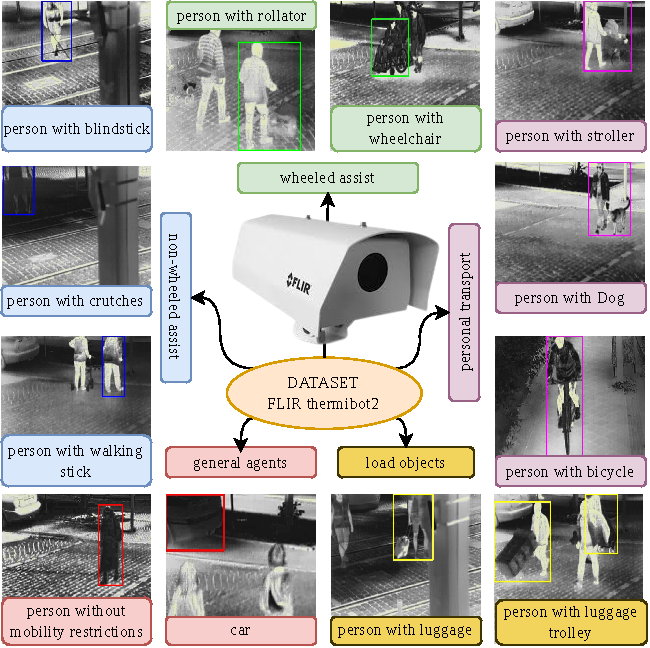
\includegraphics[width=\columnwidth]{datasetAdvik.pdf}
\caption{TMCR dataset: description for class and sub-classes}
\label{fig:yolo_images}
\end{figure}

{The main contributions of this work are:}
\begin{itemize}
    \item \textbf{Dataset for thermal mobility-context recognition:} We formulate Thermal Mobility-Context Recognition (TMCR) as a fine-grained, privacy-preserving thermal sensing problem and introduce a new FLIR ThermiBot~2 dataset organized into five mobility-context classes. %(general agents, wheeled mobility assistance, non-wheeled mobility assistance, load-bearing objects, and personal/dependent transport).
    
    \item \textbf{Thermal-aware lightweight detector design:} We propose DA-ORB YOLO that combines depthwise-efficient feature extraction with ECA~\cite{wang2020eca} and SA~\cite{bao2023sctanet} to improve thermal saliency modeling under low-contrast IR conditions while maintaining computational efficiency.
    
    \item \textbf{Resource-efficient edge deployment and validation:} We develop a cloud-edge inference framework and evaluate deployment on multiple edge platforms, including NVIDIA Jetson AGX Xavier~\cite{jetson_agx_xavier}, Raspberry Pi 5B~\cite{raspberry_pi_5}, Rock Pi 4C+~\cite{rock_pi_4c_plus}, and Raspberry Pi Zero 2W~\cite{raspberry_pi_zero_2w} demonstrating hardware scalability and practical edge feasibility for thermal sensing applications.
\end{itemize}

%The remainder of the paper is organized as follows. Section~II presents the dataset and existing YOLO architectures. Section~III details proposed YOLO architecture. Section~IV details the cloud-edge system architecture. Section~V and Section~VI reports results and conclusions, respectively.

\section{Dataset and Related Works}

\subsection{Existing Datasets}
The mobility aid dataset~\cite{vasquez2017deep,kollmitz2019deep} is one of the few benchmarks addressing people with mobility restrictions in indoor environments such as hospitals and public buildings. It provides more than 17{,}000 annotated RGB-D images while ensuring privacy through depth sensing. In contrast, for IR-based perception, most existing datasets, such as OSU~\cite{davis2007background}, FLIR ADAS~\cite{flir_adas_dataset}, KAIST~\cite{choi2018kaist}, and DENSE~\cite{bijelic2020seeing} mainly capture pedestrians or vehicles under diverse weather conditions without distinguishing between different mobility contexts as summarized in Table~\ref{tab:dataset_comparison}. The OSU dataset includes six low-resolution thermal videos of pedestrians recorded with a fixed Raytheon PalmIR 250D sensor. FLIR ADAS contains 9{,}711 thermal images across 15 object classes captured by a Teledyne FLIR Tau camera. The KAIST dataset combines thermal and visible imaging for autonomous and assisted driving and provides 8{,}970 thermal images recorded using a FLIR A655Sc camera. Similarly, the DENSE dataset integrates LiDAR, radar, and infrared data for adverse-weather driving scenarios and includes 11{,}500 thermal images captured by an Axis Q1922 FIR sensor. Although comprehensive, these datasets~\cite{davis2007background,flir_adas_dataset,choi2018kaist,bijelic2020seeing} do not include semantic differentiation of human mobility modes, which is essential for inclusive and context-aware perception. The actual dataset is Mobility-restriction data for barrier reduction at traffic-light-controlled intersections is collected in TD4PWMR~\cite{ni2025thermal}.
\begin{table}[t]
\centering
\caption{TMCR Dataset class and subclass instance counts}
\label{tab:simple4-clean}
\begin{tabular}{p{1.5cm} l l r}
\toprule
\textbf{Class} & \textbf{Total} & \textbf{Sub-Class} & \textbf{Count} \\
\midrule

\multirow{2}{=}{General Agents} & \multirow{2}{*}{14841} & person without mobility restrictions & 12117 \\ 
\cmidrule(lr){3-4}
                                &                         & car                                  & 2724 \\ 
\midrule

\multirow{2}{=}{Wheeled Mobility Assistance} & \multirow{2}{*}{1240} & person with wheelchair & 660 \\ 
\cmidrule(lr){3-4}
                                             &                        & person with rollator   & 580 \\ 
\midrule

\multirow{3}{=}{Non-Wheeled Mobility Assistance} & \multirow{3}{*}{2645} & person with crutches      & 50 \\ 
\cmidrule(lr){3-4}
                                                 &                        & person with walking stick & 97 \\ 
\cmidrule(lr){3-4}
                                                 &                        & person with blindstick    & 2498 \\ 
\midrule

\multirow{2}{=}{Load-Bearing Objects} & \multirow{2}{*}{324} & person with luggage                & 283 \\ 
\cmidrule(lr){3-4}
                                      &                        & person with shopping/luggage trolley & 41 \\ 
\midrule

\multirow{3}{=}{Personal / Dependent Transport} & \multirow{3}{*}{1377} & person with stroller & 137 \\ 
\cmidrule(lr){3-4}
                                                &                        & person with bicycle  & 1159 \\ 
\cmidrule(lr){3-4}
                                                &                        & person with dog      & 81 \\ 
\bottomrule
\end{tabular}
\end{table}

\subsection{Dataset in This Work}
A total of eight FLIR ThermiBot~2 infrared cameras were installed for dataset collection. Each camera operates within a spectral range of 7.5--13.5~$\mu$m, with a native resolution of $640 \times 512$ pixels, and supports focal lengths from 9~mm to 35~mm, enabling flexible deployment. The dataset includes 3{,}086 images captured in spring, 2{,}584 in summer, 2{,}534 in autumn, and 2{,}992 in winter. The image distribution is intentionally balanced across seasons to reduce seasonal bias during model training and evaluation. We have five semantic categories along with their corresponding subclasses. The five predefined classes are: general agents, wheeled mobility assistance, non-wheeled mobility assistance, load-bearing objects, and personal or dependent transport, as illustrated in Fig.~\ref{fig:yolo_images}. The class and subclass frequency distribution of the dataset is provided in Table~\ref{tab:simple4-clean}. For wheeled mobility assistance, the bounding box includes both the person and the wheelchair or rollator. Similarly, for strollers, bicycles, and dogs, the bounding box covers the person and the associated object. This combined labeling leverages the relative spatial relationship between the person and the item, improving detection accuracy.


\begin{comment}
    

\subsection{YOLO Developments}

The progress of modern IR object detection is closely linked to the evolution of real-time detectors. YOLOv1~\cite{redmon2016you} introduced the first CNN-based one-stage detector capable of real-time performance. Subsequent YOLO versions~\cite{lin2017focal,wang2021scaled,wang2023yolov7,li2023yolov6} progressively improved detection speed, accuracy, and scalability. Early variants (YOLOv1 to YOLOv3) established dense prediction and multi-scale detection. Later versions, such as YOLOv4, YOLOv5, and YOLOv7, integrated advanced training strategies and architectural components such as SPP, PANet, and CSP to enhance accuracy without compromising speed. YOLOv8 introduced anchor-free detection, the C2f backbone module, and a decoupled head for faster convergence. YOLOv10 focused on deployment efficiency through an end-to-end NMS-free design with dual-label assignment. YOLOv11 further improved backbone efficiency with C3k2 and C2PSA modules that combine lightweight convolutions with partial self-attention. Alongside convolution-based YOLO models, transformer-based detectors such as DETR~\cite{carion2020end} redefined object detection through end-to-end architectures that remove handcrafted anchors and non-maximum suppression. However, DETR models typically suffer from slow convergence and high computational overhead, limiting their suitability for real-time or embedded IR systems. Although recent variants such as RT-DETR attempt to reduce inference cost, lightweight and thermally optimized models remain underexplored.

Beyond backbone scaling, numerous YOLO variants incorporate custom architectural modules tailored to specific sensing conditions. Spatial and channel attention mechanisms have been used to enhance detection in thermal or low-contrast environments. Coordinate Attention~\cite{hou2021coordinate} improves localization sensitivity and has been applied in YOLOv7-CA and YOLOv8-CA for road-scene and aerial IR tasks. CBAM integrates channel and spatial attention and has been applied to thermal pedestrian detection and medical thermal imagery. ECA~\cite{wang2020eca} provides efficient channel re-weighting without dimensionality reduction, making it suitable for embedded YOLO deployments. Triplet Attention~\cite{misra2021triplet} and hybrid attention have also been utilized in YOLO-Thermal~\cite{ni2025thermal} and related IR detection frameworks to capture anisotropic thermal features. These developments show that YOLO backbones are highly task-dependent. Modules designed for visible-spectrum images are often modified or replaced when applied to infrared, medical, or aerial domains. The literature also summarizes that the choice of attention mechanisms and convolutional context must be guided by sensing modality and deployment constraints.
\end{comment}
\begin{figure*}[t]
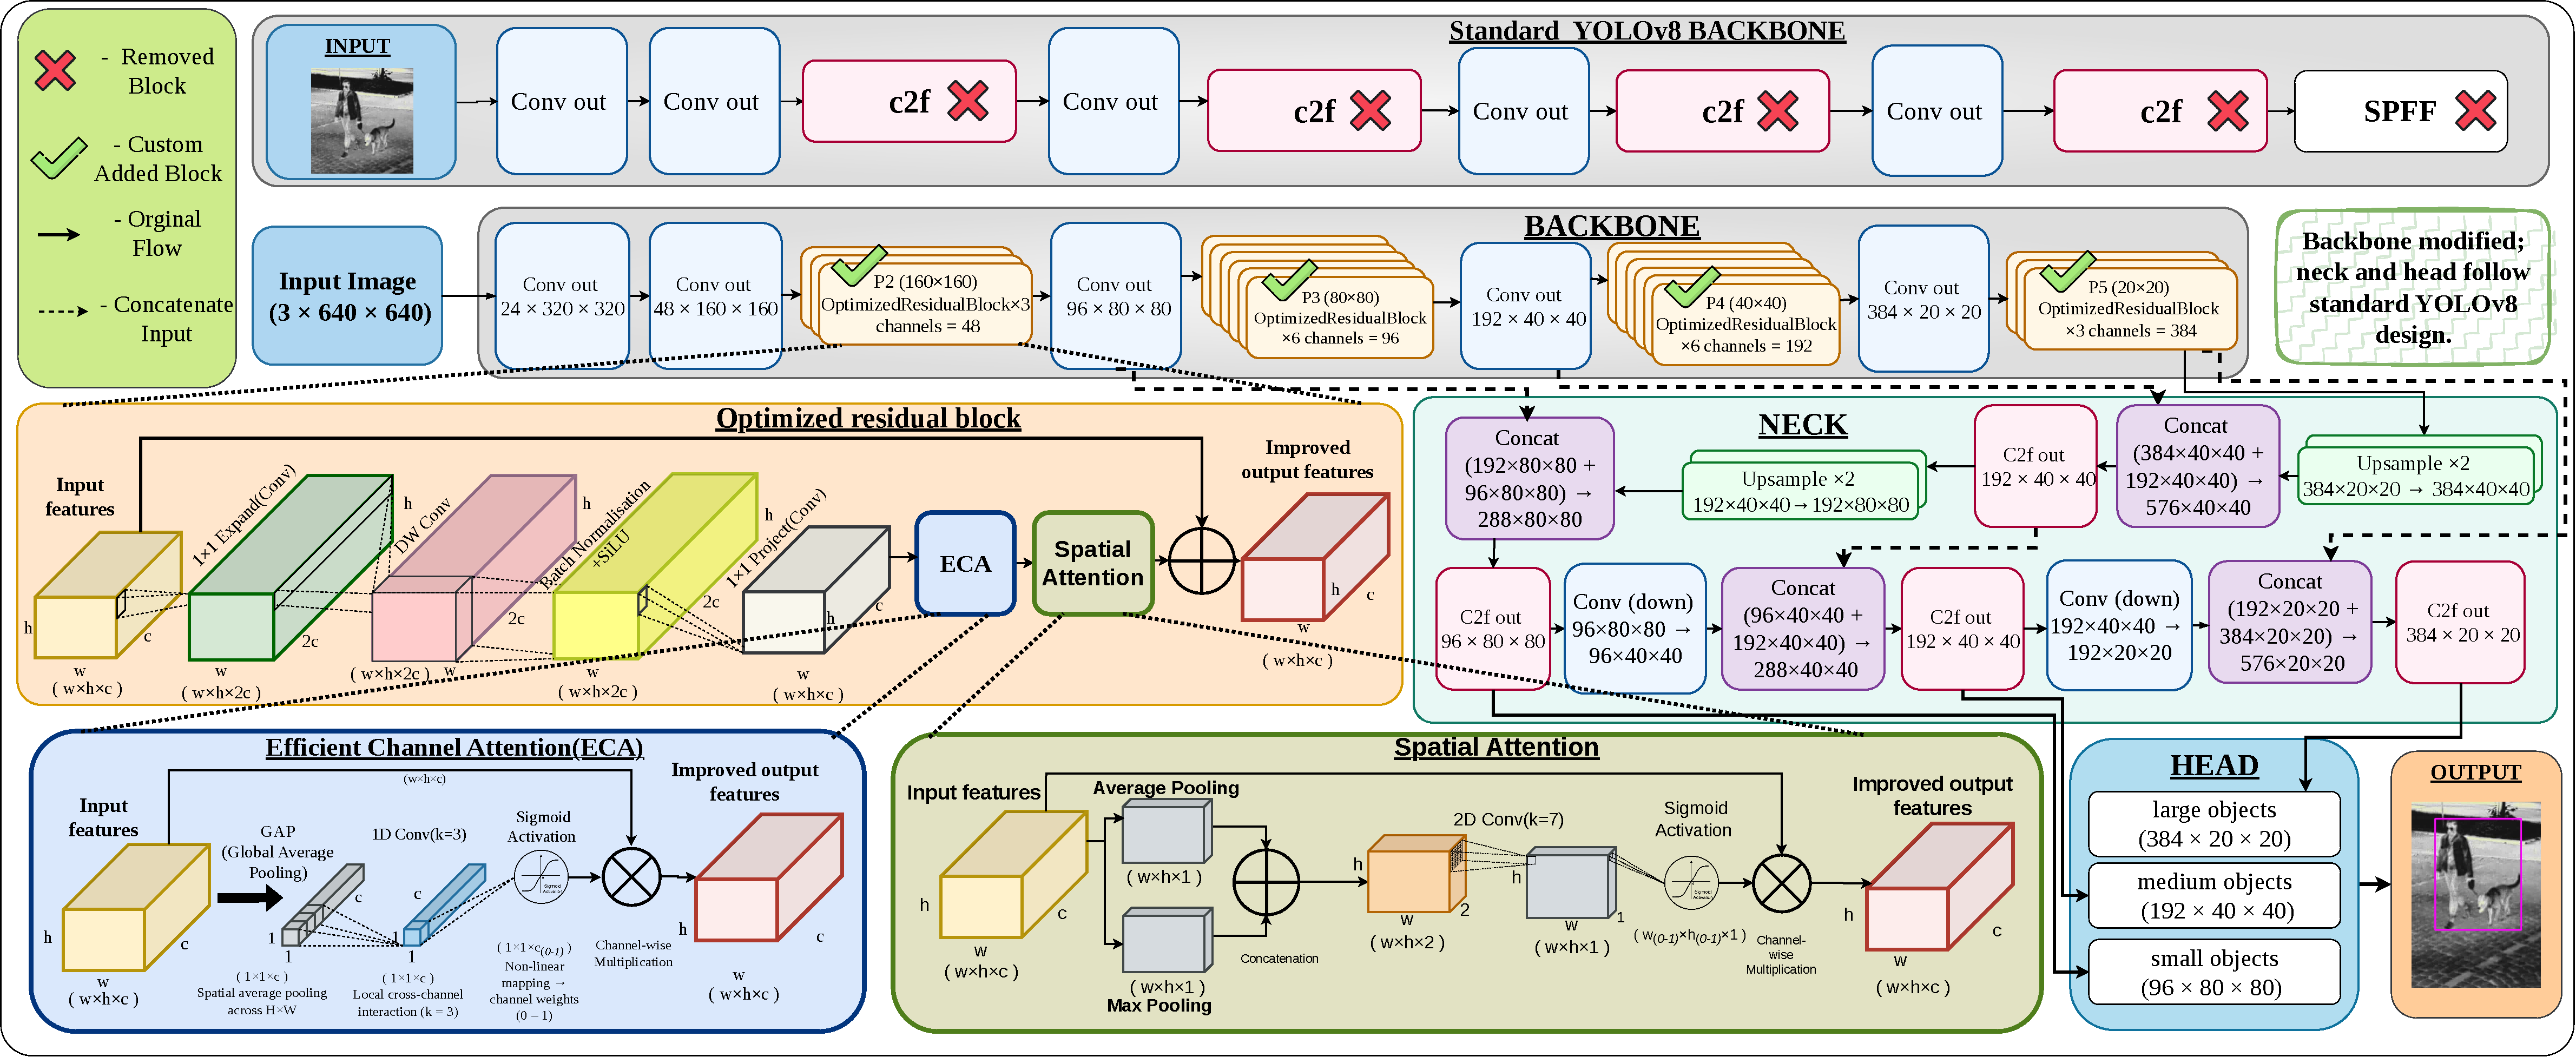
\includegraphics[width=\linewidth]{yoloarchitecture.pdf}
\caption{{Proposed custom YOLO architecture. (On the top row, we provided a standard YOLOv8  backbone with c2f blocks, and gets replaced by optimized residual block in the proposed YOLO variant)}}
\label{fig:yolo_arch}
\end{figure*}

\section{Proposed Method: Dual Attention YOLO}
\label{sec:proposed}

We introduce dual attention YOLO, a compact yet thermally adaptive object detection network. The design emphasizes discriminability through architectural refinement rather than scale expansion or heavy augmentation. At its core lies the Dual Attention Optimized Residual Block (DA-ORB), a unified computational unit that replaces the standard \texttt{C2f} block of YOLOv8. This block integrates both {Efficient Channel Attention (ECA)~\cite{wang2020eca} and Spatial Attention (SA)~\cite{bao2023sctanet} within an inverted residual structure to jointly enhance what (spectral relevance) and where (spatial saliency) representations in thermal images}.

%\subsection{Network Overview}
The proposed dual attention YOLO follows the canonical single-stage detection paradigm:

\begin{itemize}
    \item \textbf{Backbone:} Stacked DA-ORB modules progressively downsample the input thermal image to generate multi-scale feature maps $(P_1$--$P_5)$. Each block adaptively emphasizes salient channels and spatial regions corresponding to thermally discriminative cues such as body posture or assistive-device contours. This backbone differs from the standard YOLOv8 architecture.
    \item \textbf{Neck and Head:} A PANet-based neck fuses cross-scale features through bottom-up and top-down pathways, ensuring rich semantic propagation to the detection head. The detection head performs class prediction and bounding-box regression using decoupled branches. The neck and head remain identical to YOLOv8 model.
\end{itemize}

\subsection{Dual Attention Optimized Residual Block (DA-ORB)}
Each DA-ORB replaces a single \texttt{C2f} block (refer Fig.~\ref{fig:yolo_arch}) and performs expansion, depthwise convolution, projection, dual attention, and residual fusion as a single atomic operation. Let $X_{\text{in}}\in\mathbb{R}^{C\times H\times W}$ denote the input feature map. The sequence of operations is described below.

\subsubsection{Expansion and Depthwise Convolution}
This stage increases the representational capacity of the input feature map while maintaining computational efficiency. First, a pointwise ($1\times1$) convolution expands the channel dimension to enrich feature diversity. A depthwise $5\times5$ convolution is then applied to capture broader spatial context while keeping the number of parameters low. Batch normalization and SiLU activation further stabilize training and introduce non-linearity
$$U = \mathrm{BN}\!\left(\mathrm{SiLU}\!\left(\mathrm{DWConv}_{5\times5}\!\left(\mathrm{Conv}_{1\times1}(X_{\text{in}},\,C\!\rightarrow\!2C)\right)\right)\right),
$$

\subsubsection{Projection}

After feature expansion and spatial processing, the number of channels is reduced back to the original dimensionality. This projection step compresses the enriched features while preserving the most informative representations, ensuring compatibility with the residual connection.
$$
F = \mathrm{BN}\!\left(\mathrm{Conv}_{1\times1}(U,\,2C\!\rightarrow\!C)\right).
$$

\begin{algorithm}[t]
\caption{Dual Attention Optimized Residual Block}
\label{alg:daorb}
\begin{algorithmic}[1]
\REQUIRE $X_{\text{in}}\in\mathbb{R}^{C\times H\times W}$
\STATE $U \leftarrow \mathrm{BN}(\mathrm{SiLU}(\mathrm{Conv}_{1\times1}(X_{\text{in}},C\!\rightarrow\!2C)))$
\STATE $U \leftarrow \mathrm{BN}(\mathrm{SiLU}(\mathrm{DWConv}_{5\times5}(U)))$
\STATE $F \leftarrow \mathrm{BN}(\mathrm{Conv}_{1\times1}(U,2C\!\rightarrow\!C))$
\STATE $z \leftarrow \mathrm{GAP}(F)$
\STATE $\omega \leftarrow \sigma(\mathrm{Conv1D}_k(z))$
\STATE $F_{\text{eca}} \leftarrow \omega \otimes F$
\STATE $F_{\text{avg}} \leftarrow \mathrm{AvgPool}(F_{\text{eca}})$, \quad $F_{\text{max}} \leftarrow \mathrm{MaxPool}(F_{\text{eca}})$
\STATE $M_{\text{sa}} \leftarrow \sigma(\mathrm{Conv}_{7\times7}([F_{\text{avg}};F_{\text{max}}]))$
\STATE $F_{\text{sa}} \leftarrow M_{\text{sa}} \otimes F_{\text{eca}}$
\STATE $X_{\text{out}} \leftarrow X_{\text{in}} + F_{\text{sa}}$
\RETURN $X_{\text{out}}$
\end{algorithmic}
\end{algorithm}

\subsubsection{Efficient Channel Attention (ECA)}

To emphasize informative channels and suppress less relevant ones, an Efficient Channel Attention (ECA) mechanism is applied. This module models local cross-channel dependencies without dimensionality reduction, allowing the network to adaptively recalibrate channel responses based on global contextual information.

Global average pooling produces channel descriptors as $z = \mathrm{GAP}(F), \qquad z\in\mathbb{R}^{C}$. These channel descriptors summarize global spatial information for each feature channel, serving as compact statistics for attention computation.

Local cross-channel interaction is modeled using a 1-D convolution as $
\omega = \sigma(\mathrm{Conv1D}_k(z))$,
where $k$ is adaptively determined by the channel dimensionality. The channel-refined tensor is $
F_{\text{eca}} = \omega \otimes F$. This attention weighting strengthens channels that carry meaningful infrared cues while reducing the influence of less informative responses. ECA recalibrates each channel based on local cross-correlations without dimensionality reduction, making it suitable for IR-specific feature enhancement.

\subsubsection{Spatial Attention (SA)}
While channel attention focuses on \emph{what} features are important, spatial attention determines \emph{where} important information is located within the feature map. This mechanism helps highlight thermally salient regions that correspond to meaningful objects or structures in infrared imagery.

Average and maximum pooling across channels yields $
F_{\text{avg}}=\mathrm{AvgPool}(F_{\text{eca}})$ and $F_{\text{max}}=\mathrm{MaxPool}(F_{\text{eca}})$, respectively. These pooled maps capture complementary contextual information, where average pooling reflects overall activation patterns and max pooling emphasizes the most prominent responses.

The concatenated map is processed by a $7\times7$ convolution as
$
M_{\text{sa}} = \sigma(\mathrm{Conv}_{7\times7}([F_{\text{avg}};F_{\text{max}}]))$. Finally, the spatially refined output is
$
F_{\text{sa}} = M_{\text{sa}} \otimes F_{\text{eca}}$.
SA highlights thermally salient regions such as mobility aids or object boundaries, addressing the low-texture limitations of FIR imagery.

\subsubsection{Residual Fusion}
Finally, the refined features are fused with the original input through a residual connection. This design preserves the initial information flow while enabling the network to learn residual feature refinements, improving gradient propagation and model stability.

The refined features are added to the shortcut path:
\begin{equation}
X_{\text{out}} = X_{\text{in}} + F_{\text{sa}}.
\label{eq:residual}
\end{equation}

DA-ORB modules can directly replace \texttt{C2f} layers in YOLOv8 or YOLOv10 backbones while maintaining full compatibility with the PANet neck and decoupled detection head. Embedding DA-ORB modules across the backbone enables the network to exploit subtle thermal contrasts and spatial cues inherent in human-object interactions. Unlike heavier architectures, the proposed design remains suitable for embedded edge platforms such as Jetson AGX Xavier, Raspberry~Pi~5B, Raspberry~Pi~Zero~2W, and Rock~Pi~4C+.

\begin{figure*}[t]
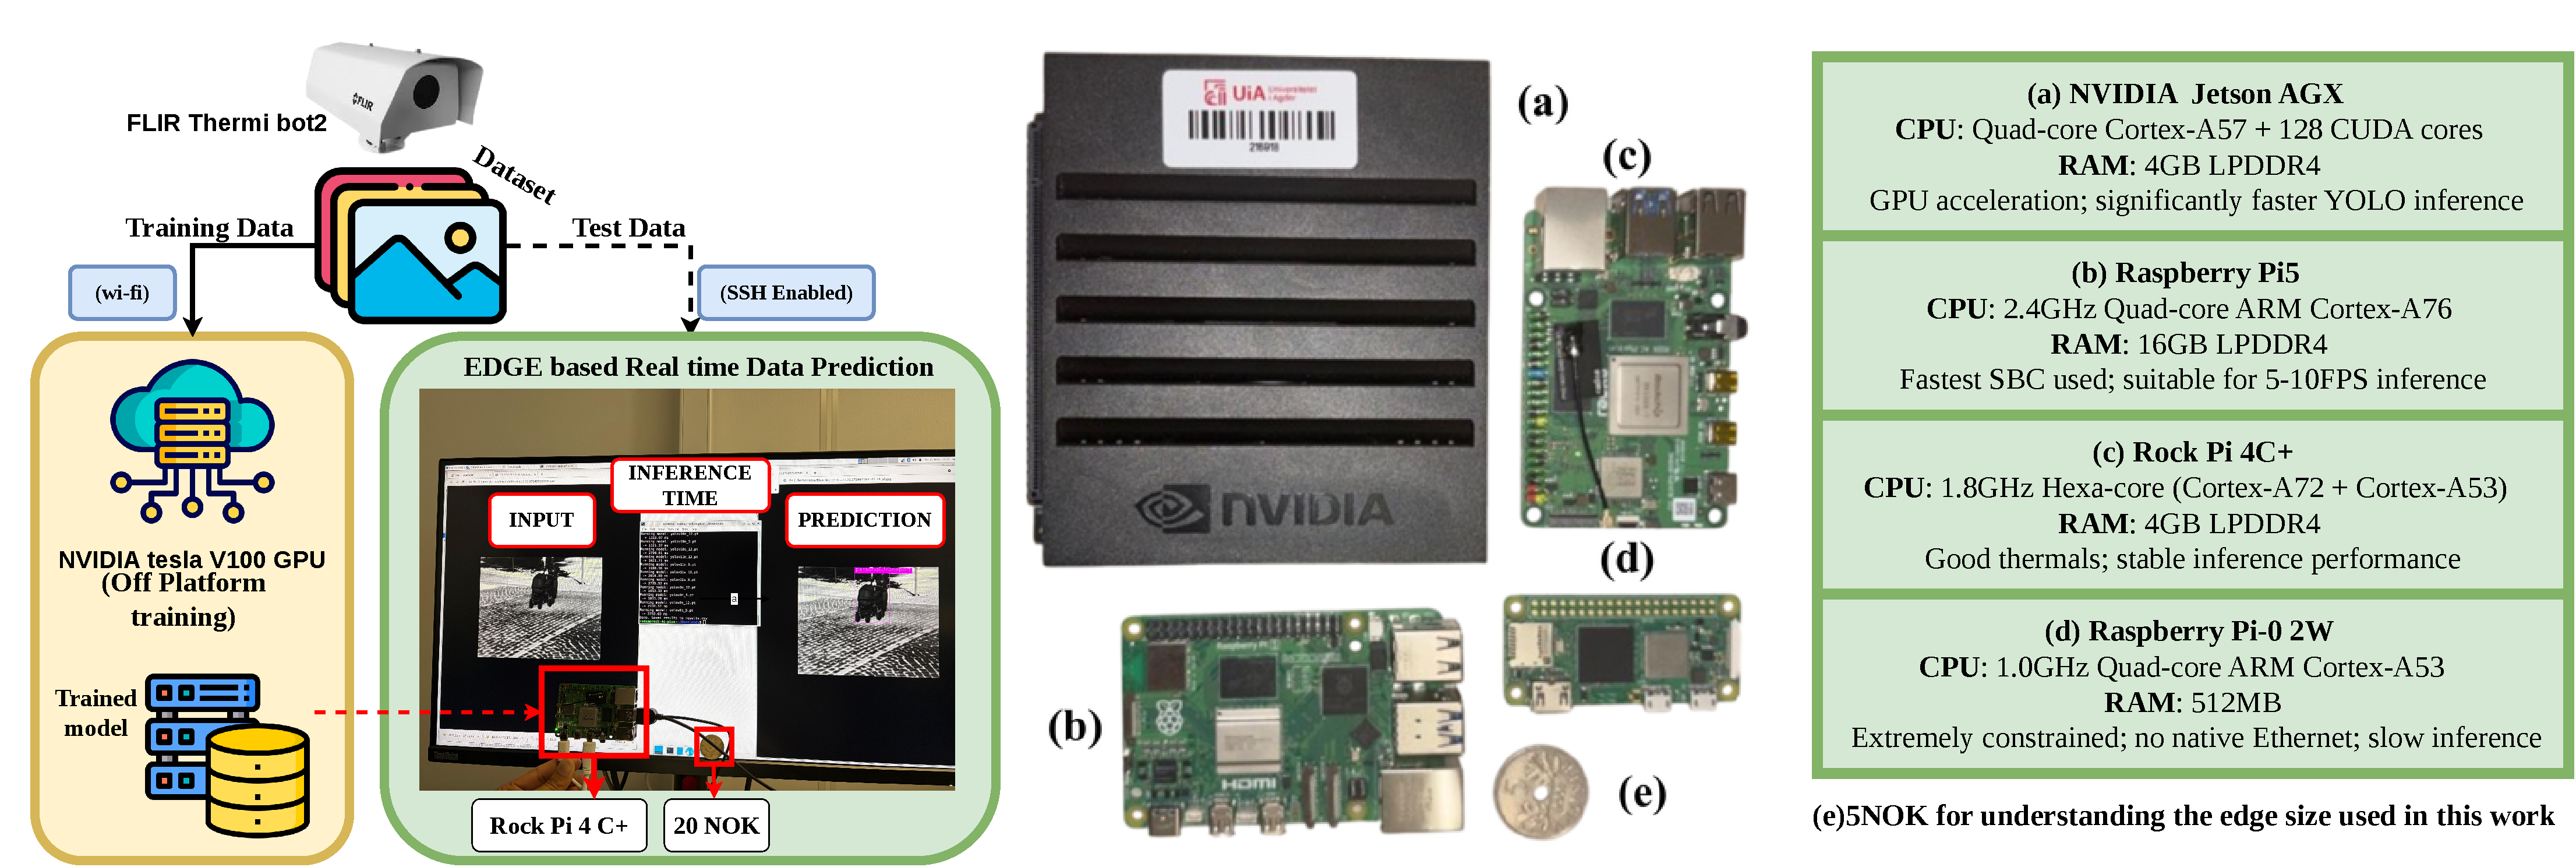
\includegraphics[width=\textwidth]{yolo_thermal_edge_explanation.drawio.pdf}
\caption{{The training and inference chain used in the proposed work. The left most figure depicts the proposed cloud-edge framework; the edge modules used in this work are (a) NVIDIA Jetson AGX Xavier~\cite{jetson_agx_xavier}, (b) Raspberry Pi 5B~\cite{raspberry_pi_5}, (c) Rock Pi 4C+~\cite{rock_pi_4c_plus}, (d) Raspberry Pi Zero 2W~\cite{raspberry_pi_zero_2w}, and (e) 5 NOK coin to understand the size of edge modules used in this work.}}
\label{fig:edge}
\end{figure*}


\subsection{Two-Stage Training Strategy}
Training from randomly initialized weights requires a high initial learning rate for the network to learn foundational features and escape a chaotic state. However, although a high learning rate accelerates early learning, it can prevent convergence by causing the optimization to overshoot the optimal solution. Conversely, starting with a low learning rate results in slow and inefficient early training. Since the proposed model is trained from scratch without pre-trained weights, we adopt a two-stage training strategy to balance stability and final precision.

Stage~1 uses a relatively high learning rate to establish a strong feature foundation, allowing the model to quickly learn general object characteristics. Stage~2 then uses a significantly lower learning rate to refine the learned representation with higher precision. The hyperparameters for both stages are summarized in Table~\ref{tab:hyperparameters}. %In Stage~1, the AdamW optimizer is used with an initial learning rate of $0.01$, a final learning rate of $0.0001$, and cosine annealing. In Stage~2, the initial and final learning rates are $0.002$ and $0.00005$, respectively. This fine-tuning phase enables small and stable updates, helping the model converge to a deeper loss minimum and achieve the high-precision localization and classification required for the mAP@50--95 metric.


\begin{table}[t]
\centering
\caption{Summary of two-stage training hyperparameters}
\label{tab:hyperparameters}
\begin{tabular}{p{3cm} p{2.4cm} p{2cm}}
\toprule
{Parameter} & {Stage-1 } & {Stage-2 } \\
 & \textbf{Foundation} & \textbf{Refinement} \\
\midrule
Epochs & 200 & 150 \\
Image Size & 640x640 & 640x640 \\
Batch Size & 16 & 12 \\
Optimizer & AdamW & AdamW \\
Initial Learning Rate ($\text{lr0}$) & 0.01 & 0.002 \\
Final Learning Rate ($\text{lrf}$) & 0.0001 & 0.00005 \\
Cosine Annealing & True & True \\
Warmup Epochs & 10 & 5 \\
Momentum & 0.937 & 0.95 \\
Weight Decay & 0.0005 & 0.0001 \\
Loss Weight (box) & 7.5 & 8.5 \\
Loss Weight (cls) & 0.5 & 0.4 \\
Loss Weight (dfl) & 1.5 & 1.8 \\
Augmentation & False & False \\
\bottomrule
\end{tabular}
\end{table}



\begin{table*}[t]
\centering
\caption{{Pretrained YOLO model on COCO dataset + retrain using accumulated TMCR dataset. Values are written as ``no-augmentation (augmentation)'' to explain the impact of thermal image augmentation on model prediction.}}
\label{tab:merged_yolo_comparison_transfer}
\small
\renewcommand{\arraystretch}{1.15}
\begin{tabular}{l c c c c c c c}
\toprule
{\textbf{Model}} & {\textbf{Params (M)}} & {\textbf{GFLOPs}} &
{\textbf{Precision (\%)}} & {\textbf{Recall (\%)}} & {\textbf{mAP@50 (\%)}} &
{\textbf{mAP@50--95 (\%)}} & {\textbf{Size (MB)} }\\
\midrule

{YOLOv8n}  & {3.1}  & {8.8}  &
{95.73 (94.02)} & {93.45 (93.97)} & {97.04 (96.99)} & {90.34 (89.54)} & {6} \\

{YOLOv8s}  & {11.1}  & {28.8 } &
{97.86 (96.36) }& {92.69 (94.57) }&{ 97.42 (97.43)} & {91.78 (92.10)} &{ 21.5 }\\

{YOLOv10n}  & {2.7}  & {8.7}  &
{95.480 (95.28) }&{ 93.029 (91.07)} & {97.087 (95.88)} &{ 89.633 (88.66)} & {5.5} \\

{YOLOv10s}  & {8.1}  & {25.1}  &
{93.736 (95.36)} & {92.969 (88.43)} & {96.426 (95.39)} & {88.020 (86.21)} & {15.8} \\

{YOLOv11n}  & {2.6}  & {6.6}  &
{96.48 (95.64)} & {91.22 (91.91)} & {97.01 (96.96)} & {90.39 (89.14)} & {5.2} \\

{YOLOv11s}  & {9.1}  & {25.5}  &
{94.63 (96.12)} & {95.13 (94.11)} & {97.17 (97.48)} & {90.62 (91.39)} & {18.3} \\

\bottomrule
\end{tabular}
\end{table*}


\begin{table*}[t]
\centering
\caption{Comparison of existing YOLO and the proposed model on the TMCR dataset.}
\label{tab:merged_yolo_comparison}
\begin{tabular}{l c c c c c c c}
\toprule
\textbf{Model} & \textbf{Params (M)} & \textbf{GFLOPs} &
\textbf{Precision (\%)} & \textbf{Recall (\%)} & \textbf{mAP@50 (\%)} &
\textbf{mAP@50--95 (\%)} & \textbf{Size (MB)} \\
\midrule

YOLOv8n  & 3.1  & 8.8  & 97.09 & 91.07 & 96.63 & 88.89 & 6 \\

YOLOv8s  & 11.1  & 28.8  & 96.06 & 82.91 & 93.08 & 84.66 & 21.5 \\

YOLOv10n  & 2.7  & 8.7  & 94.31 & 91.81 & 96.25 & 88.35 & 5.5 \\

YOLOv10s  & 8.1  & 25.1  & 94.23 & 90.38 & 95.53 & 85.77 & 15.8\\

YOLOv11n  & 2.6  & 6.6  & 95.87 & 91.32 & 96.41 & 86.42 & 5.2 \\

YOLOv11s  & 9.1  & 25.5  & 93.59 & 91.10 & 95.50 & 84.31 & 18.3\\

{YOLO-SMUG~\cite{luo2025yolo} }& {7.1 } &{ 32.5} &{ 96.628 }& {91.04} &{96.35} &{ 87.20}& {xx }\\

{YOLO-CCS~\cite{li2024yolo} }  & {6.5 }   &{ 8.1 } & {92.43 }& {89.72 }& {94.09 }&{ 81.96}& {xx }\\
\midrule
\rowcolor{cyan!10}
\textbf{OURS}& \textbf{4.9}  &\textbf{15.1}&\textbf{95.1} & \textbf{93.0} & \textbf{96.6} &  \textbf{89.9} & \textbf{9.8}\\
\rowcolor{cyan!10}
{OURS + MSGF-TIR~\cite{li2024thermal} }& {4.9} &{ 15.1} &{ 96.1}   & {93.1 }  & {96.6 }  &{ 90.1 }& {{9.8}}\\
\rowcolor{cyan!10}
{OURS + KBHE~\cite{mudavath2025person}  }   & {4.9} & {15.1 }&{ 94.7}   & {92.1  } & {97.1 }  & {89.7} & {{9.8}}\\
\bottomrule
\end{tabular}
\end{table*}

\begin{table}[t]
\centering
\caption{TMCR dataset: per-category performance.}
\label{tab:tmcr category_results}
\sisetup{
  round-precision = 3,
  table-number-alignment = center
}
\begin{tabular}{
    l
    S[table-format=1.3]  % P
    S[table-format=1.3]  % R
    S[table-format=1.3]  % mAP@50
    S[table-format=1.3]  % mAP@50-95
}
\toprule
\textbf{Category} &
\textbf{P} &
\textbf{R} &
\textbf{mAP@50} &
\textbf{mAP@50-95} \\
\midrule
General agents         & 0.977 & 0.960 & 0.989 & 0.920 \\
Wheeled assist         & 0.961 & 0.940 & 0.983 & 0.926 \\
Non-wheeled assist    & 0.987 & 0.952 & 0.991 & 0.928 \\
Load objects           & 0.925 & 0.900 & 0.921 & 0.875 \\
Personal transport     & 0.905 & 0.899 & 0.947 & 0.847 \\
\midrule
\textbf{mean (mAP)}     & 0.951 & 0.930 & \bfseries 0.966 & \bfseries 0.899 \\
\bottomrule
\end{tabular}
\end{table}

\section{System Architecture and Edge Deployment}
\label{sec:cloud_edge}

This work employs a cloud-edge co-design strategy for efficient TMCR, addressing embedded hardware's computational limits. The architecture separates high-compute model training from low-latency inference at the sensing edge, as shown in Fig.~\ref{fig:edge}. The cloud is excluded from the inference loop. It handles tasks like dataset management, annotation, and model training, while the embedded device executes the lightweight detection model locally. This design aligns with best practices in intelligent sensing systems, where training is centralized for efficiency and inference is decentralized for responsiveness and autonomy. The cloud-edge pipeline transforms a conventional thermal camera into an intelligent, resource-efficient sensing node.

%This work adopts a cloud-edge co-design strategy to enable efficient TMCR while addressing the computational limitations of embedded hardware. The architecture separates the high-compute stages of model training from the low-latency inference required at the sensing edge, as shown in Fig.~\ref{fig:edge}. The cloud is intentionally excluded from the inference loop. While the cloud performs computationally expensive tasks such as dataset management, annotation, and model training, the embedded device executes the lightweight detection model locally. This design follows best practices in intelligent sensing systems, where training is centralized for efficiency and inference is decentralized for responsiveness and autonomy. The cloud-edge pipeline effectively transforms a conventional thermal camera into an intelligent, resource-efficient sensing node.

\subsection{Training Pipeline (Cloud Stage)}
ThermiBot~2 infrared cameras support stable Ethernet connectivity via RTSP/HTTP streams and vendor-provided cloud access~\cite{flir_thermibot2}. Thermal data are acquired using these cameras and uploaded to a cloud server for storage, annotation, and model training. Image annotation is performed using the Roboflow platform. This work evaluates several edge devices, including Raspberry~Pi~5, Rock~Pi~4C+, Raspberry~Pi~0, Jetson AGX Xavier, to ensure comprehensive edge benchmarking. The size and specifications of these devices are shown in Fig.~\ref{fig:edge}.

Embedded devices such as Raspberry~Pi~0 do not possess sufficient memory or processing capability to train YOLO models and also lack the peripheral support needed for convenient training workflows. Therefore, all training operations, including backbone learning, attention-module optimization, and weight updates, are executed entirely in the cloud using GPU resources.

All experiments were conducted on a workstation equipped with an NVIDIA Tesla V100-SXM3-32GB GPU. The models were implemented using PyTorch v2.8.0 and the Ultralytics v8.3.203 framework. After training, the Dual Attention YOLO model is exported as a lightweight checkpoint file (e.g., \texttt{.pt}). This file is transferred once to the edge device as part of the deployment process and is not involved in the real-time inference path.

\subsection{Inference Pipeline (Edge Stage)}
During deployment, thermal frames from the ThermiBot~2 camera stream to the edge device. For example, on the Raspberry~Pi, the downloaded model checkpoint loads from local storage, and all inference operations are on-device. This ensures low-latency detection without cloud dependency. Local inference offers advantages like real-time processing without network delays, improved privacy as raw thermal data stays on site, and low-power operation for resource-constrained installations.
%During deployment, thermal frames from the ThermiBot~2 camera stream directly to the edge device. For example, on the Raspberry~Pi, the previously downloaded model checkpoint is loaded from local storage, and all inference operations are performed on-device. This ensures low-latency detection without any dependency on cloud connectivity. Local inference provides several advantages, including real-time processing without network delays, improved privacy since raw thermal data never leaves the site, and low-power operation suitable for resource-constrained installations.

% --- SECTION 4: EXPERIMENTS ---
\section{Experiments and Results}
\subsection{Comparison with State-of-the-Art: TMCR Dataset}

To validate the effectiveness of the proposed architecture, we conducted a comprehensive comparison against a range of lightweight YOLO models (nano- and small-scale). {We first considered the publicly available pretrained models (trained on the COCO dataset) and then retrained them on the TMCR dataset, both with and without data augmentation. The results, summarized in Table~\ref{tab:merged_yolo_comparison_transfer}, show that augmentation does not provide accuracy gains for thermal imagery. This is consistent with the low-texture nature of FIR data, where synthetic perturbations tend to distort the underlying thermal patterns rather than improve generalization. We do not claim that fine-grained mobility-context recognition is entirely absent from the broader literature, nor that existing object detection frameworks cannot be adapted to such classes. Rather, this work focuses on the underexplored combination of thermal sensing, fine-grained mobility-context categorization, and resource-constrained edge deployment.}


To ensure a fair architectural comparison, we then trained all competing models entirely from scratch on the TMCR dataset, without pretraining or augmentation. Under these identical conditions, our \textit{Dual Attention YOLO} achieves the highest overall accuracy, reaching 89.9\% mAP@50--95. This is a substantial improvement over the closest lightweight baselines, including YOLOv8n (88.89\% mAP@50--95) and YOLOv10n (88.35\% mAP@50--95). {In addition, we considered thermal YOLo varient of YOLO-SMUG (ShuffleNetV2 + Multi-Scale Dilated Attention + Universal Inverted Bottleneck + GhostConv)~\cite{luo2025yolo} and YOLO-CCS (Coordinate Attention + C2f module + SIOU loss)~\cite{li2024yolo} custom thermal architecture from the literature to show the competence of the proposed model. Wherein we observed both~\cite{luo2025yolo} and~\cite{li2024yolo} are bulky models. Also, for thermal datasets, the pre-processing place a crucial role in detection. To evaluate it, we consider two popular and existing pre-processing techniques from literature namely multi-scale guided filtering based thermal infrared (MSGF-TIR)~\cite{li2024thermal} and kurtosis based histogram enhancement(KBHE)~\cite{mudavath2025person}. The dataset is processed through the pre-processing module and repeated the experiment, we observed that MSGF-TIR~\cite{li2024thermal} enhances the accuracy of the model.} These results provide strong evidence that the proposed \texttt{OptimizedResidualBlock} with integrated ECA and SA attention mechanisms provides superior thermal feature learning compared to standard YOLO backbones.

For a finer analysis, Table~\ref{tab:merged_yolo_comparison} reports the per-class metrics of our final trained model. The detector achieves exceptionally high performance on common categories such as \texttt{general agents} (mAP@50 = 0.989) and \texttt{non-wheeled assist} (mAP@50 = 0.991). More importantly, the network maintains strong accuracy on the challenging fine-grained thermal classes that are central to the TMCR dataset. For example, the model obtains 92.6\% mAP@50--95 on \texttt{wheeled assist} and 84.7\% mAP@50--95 on \texttt{personal transport}, demonstrating its ability to distinguish subtle thermal cues associated with wheelchairs, strollers, dogs, and bicycles under low-contrast FIR conditions. These results confirm that the proposed Dual Attention YOLO is not only lightweight but also significantly more thermally discriminative than existing YOLO variants, making it a strong candidate for real-time mobility-context recognition on embedded devices
\begin{table}[t]
\caption{{Cross-dataset performance of the proposed model on established thermal and related perception benchmarks.}}
\label{tab:dataset_results}
\centering
\resizebox{\columnwidth}{!}{
\begin{tabular}{lrrrrrrr}
\hline
{\textbf{Dataset}}  & {\textbf{Precision}} & {\textbf{Recall}} & {\textbf{mAP50}} & {\textbf{mAP50-95}} & {\textbf{GFLOPs}} \\
\hline
{ITDAV-25~\cite{hbje-ef33-25}}       & {0.967} & {0.956} & {0.976} & {0.860} & {15.1} \\
{OSU Thermal~\cite{davis2007background}}    & {0.990} & {0.951} & {0.989} & {0.761} & {15.0} \\
{C3I Thermal~\cite{jf21-rt22-22}}  & {0.918} & {0.882} & {0.928} & {0.608} & {15.1} \\
{OSU Colour~\cite{osu_color_dataset}}      & {0.980} & {0.938} & {0.960} & {0.754} & {15.0} \\
{FLIR\_ADAS\_v2~\cite{flir_adas_dataset}}  & {0.863} & {0.589} & {0.687} & {0.472} & {16.2} \\
{TD4PWMR~\cite{ni2025thermal}}  & {0.966} & {0.918} & {0.963}& {0.905} &{15.1} \\
{TMCR (Ours)} &{0.951} & {0.930}& {0.966}& {0.899} &{15.1} \\
\hline
\end{tabular}
}
\end{table}


\begin{comment}
\begin{table*}[t]
\centering
\caption{Comparison of existing YOLO and proposed model on the TD4PWMR~\cite{ni2025thermal} dataset (12 mobility classes).  NR indicates not reported in~\cite{ni2025thermal} on TD4PWMR dataset.}
\label{tab:merged_yolo_12comparison}
\begin{tabular}{l c c c c c c c}
\toprule
\textbf{Model} & \textbf{Params (M)} & \textbf{GFLOPs} &
\textbf{Precision (\%)} & \textbf{Recall (\%)} & \textbf{mAP@50 (\%)} &
\textbf{mAP@50--95 (\%)} & \textbf{Size (MB)} \\
\midrule

YOLOv8n  & 3.1  & 8.8  & 95.35 & 87.46 & 92.52 & 85.89 & 6 \\
YOLOv8s  & 11.1 & 28.8 & 94.31 & 86.83 & 92.44 & 86.53 & 21.5 \\
YOLOv10n & 2.7  & 8.7  & 97.34 & 84.73 & 93.59 & 87.61 & 5.5\\
YOLOv10s & 8.1  & 25.1 & 90.81 & 82.66 & 89.70 & 82.81 & 15.8\\
YOLOv11n & 2.6  & 6.6  & 94.66 & 87.55 & 92.09 & 85.67 & 5.2\\
YOLOv11s & 9.1  & 25.5 & 86.48 & 85.53 & 87.83 & 81.07 & 18.3 \\
YOLOv6n  & 4.2  & 11.2 & 85.77 & 83.91 & 87.33 & 81.12 & 8.3 \\
YOLOv6s  & 17.2 & 44.2 & 89.45 & 79.77 & 88.61 & 79.12 & 31.3 \\
\cite{ni2025thermal}   &42.1& 150.1&NR&NR&95.1&71.5 &NR \\
\rowcolor{cyan!10}
\textbf{Ours} &
\textbf{4.9} & \textbf{15.1} &
\textbf{96.60} & \textbf{91.80} & \textbf{96.30} & \textbf{90.50} & \textbf{9.8} \\

\bottomrule
\end{tabular}
\end{table*}
\end{comment}

\begin{comment}
\subsection{Comparison with State-of-Art: TD4PWMR Dataset}

The TD4PWMR dataset shares the same twelve subclasses as the TMCR dataset, with consistent labeling as summarized in Table~\ref{tab:simple4-clean}. To assess the generalization capability of the proposed model, we evaluate Dual Attention YOLO on the TD4PWMR dataset and compare it against existing lightweight YOLO variants as well as the YOLO-Thermal model proposed in~\cite{ni2025thermal}. The consolidated performance of all models is reported in Table~\ref{tab:merged_yolo_12comparison}. Across all metrics, our model demonstrates clear superiority. Dual Attention YOLO achieves an mAP@50 of 0.963 and an mAP@50--95 of 0.905, outperforming YOLOv8n (0.9552 / 0.858), YOLOv10n (0.935 / 0.876), and YOLOv11n (0.920 / 0.856). Even when compared with the heavier YOLO-Thermal architecture of~\cite{ni2025thermal}, which relies on YOLOv8-L with Triplet Attention, SPD-Conv, SPPFCSPC, and QFL loss; our lightweight model still achieves competitive or superior accuracy while using only a fraction of the computational budget. YOLO-Thermal~\cite{ni2025thermal} reports 93\% mAP@75, whereas our Dual Attention YOLO attains 89.1\% mAP@50--95 with only 4.9M parameters and 15.1 GFLOPs, making it substantially more efficient for embedded thermal deployments.
\begin{table}[t]
\centering
\caption{Per-class performance of the proposed YOLO on TD4PWMR~\cite{ni2025thermal}.}
\label{tab:per_class_results12}

\begin{tabular}{
    p{2.65cm}   % shortened class column to fit a single column
    S[table-format=1.3]
    S[table-format=1.3]
    S[table-format=1.3]
    S[table-format=1.3]
}
\toprule
\textbf{Class} &
\textbf{P} &
\textbf{R} &
\textbf{mAP@50} &
\textbf{mAP@50--95} \\
\midrule

person (no mobility)      & 0.982 & 0.944 & 0.987 & 0.916 \\
wheelchair                & 0.971 & 0.963 & 0.989 & 0.945 \\
rollator                  & 0.991 & 0.941 & 0.981 & 0.919 \\
crutches                  & 0.939 & 1.000 & 0.995 & 0.937 \\
blindstick                & 0.981 & 0.980 & 0.993 & 0.930 \\
luggage                   & 0.980 & 0.866 & 0.938 & 0.893 \\
stroller                  & 1.000 & 0.840 & 0.955 & 0.894 \\
bicycle                   & 0.971 & 0.860 & 0.964 & 0.868 \\
shopping trolley          & 0.940 & 1.000 & 0.995 & 0.970 \\
dog                       & 0.887 & 0.715 & 0.832 & 0.726 \\
walking stick             & 0.955 & 0.920 & 0.936 & 0.877 \\
car                       & 0.994 & 0.987 & 0.995 & 0.988 \\
\midrule
\textbf{Average}          & 0.966 & 0.918 & \textbf{0.963} & \textbf{0.905} \\
\bottomrule
\end{tabular}
\end{table}

To further interpret per-class performance, Table~\ref{tab:per_class_results12} presents the breakdown across all twelve mobility categories. The model achieves high accuracy on common categories such as \texttt{person} (mAP@50 = 0.987) and \texttt{car} (0.995). More importantly, it maintains strong performance on fine-grained mobility-related classes, achieving 99.3\% mAP@50--95 on \texttt{blindstick} and 99.5\% on \texttt{crutches}. These results confirm that the proposed architecture effectively distinguishes subtle infrared signatures in the TD4PWMR dataset. Overall, the TD4PWMR evaluation demonstrates that Dual Attention YOLO generalizes robustly across thermal datasets and consistently outperforms both lightweight and large-scale YOLO variants. Its combination of high accuracy and extremely low computational cost makes it a strong candidate for real-time thermal mobility-context recognition on resource-constrained platforms.    
\end{comment}

\begin{figure*}[t]
    \centering
    \subfloat[Box regression loss]{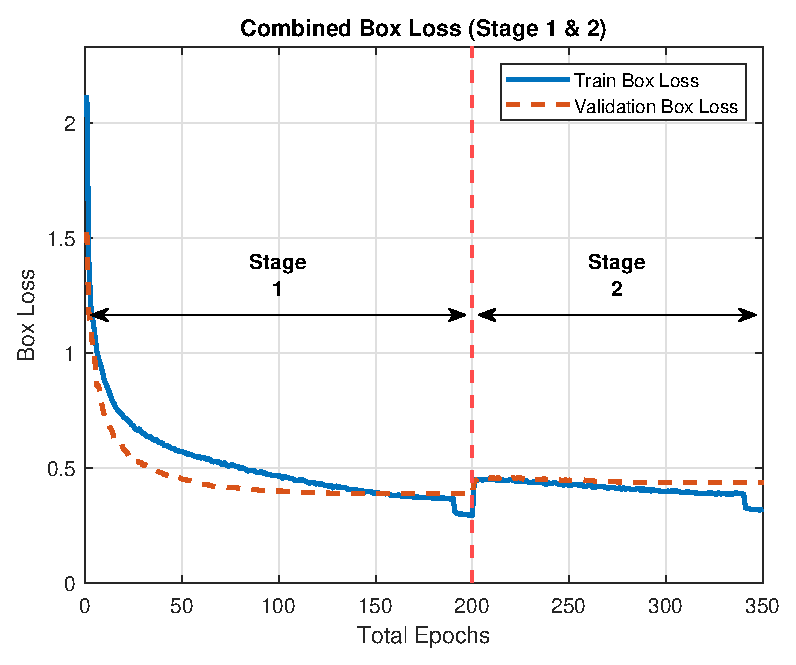
\includegraphics[width=0.24\textwidth]{combined_plot_box_loss.eps}}
    \subfloat[Classification loss]{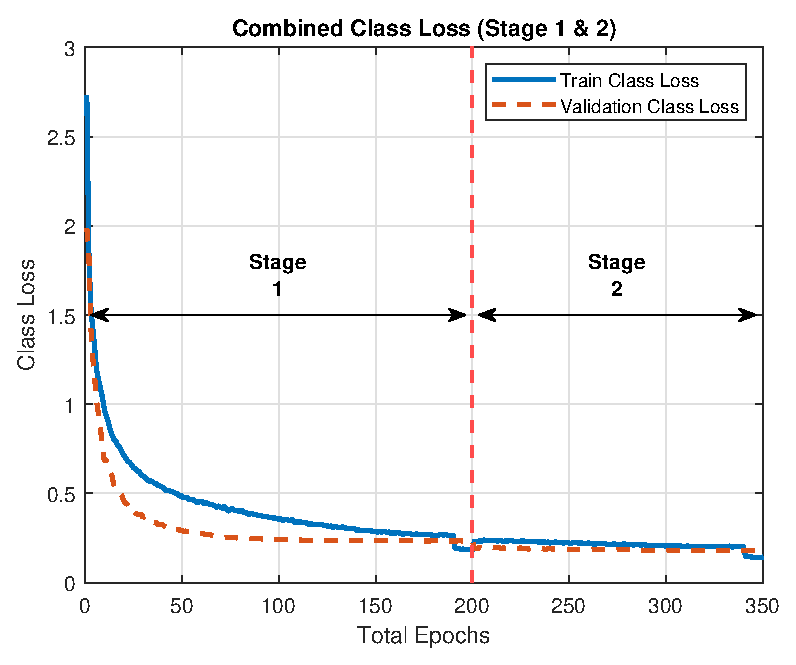
\includegraphics[width=0.24\textwidth]{combined_plot_class_loss.eps}}
    \subfloat[Precision--Recall evolution]{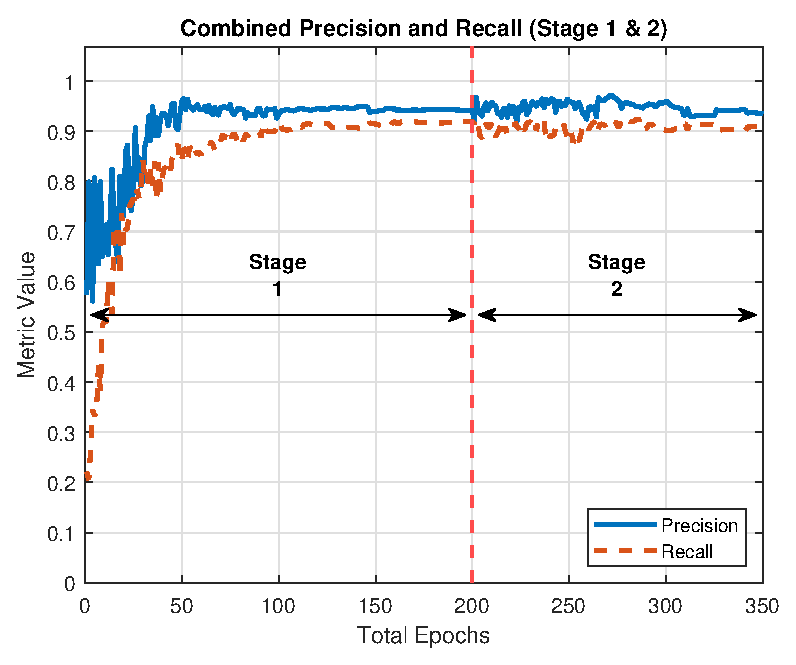
\includegraphics[width=0.24\textwidth]{combined_plot_pr.eps}}
    \subfloat[mAP progression]{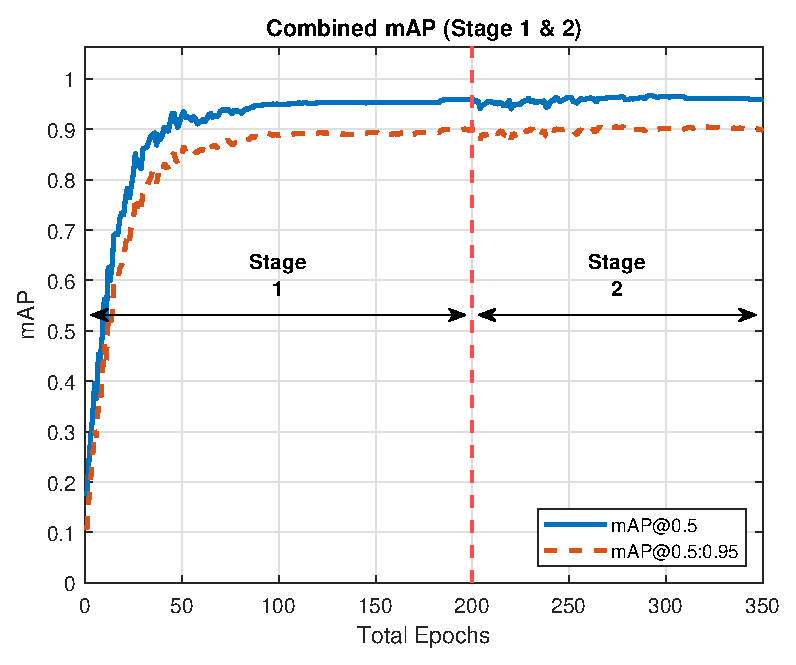
\includegraphics[width=0.24\textwidth]{combined_plot_map.eps}}
    \caption{Training dynamics of the proposed Dual Attention YOLO under the two-stage learning schedule. }
    \label{fig:training_graphs}
\end{figure*}















\begin{table*}[t]
\centering
\caption{{Inference time across servers and edge devices for mobility datasets values provided as ``TD4PWMR (TMCR)"} }
\label{tab:combined_inference_landscape}

\resizebox{\textwidth}{!}{
\begin{tabular}{lccccccc}
\toprule
\textbf{Model} &
\textbf{Intel Xeon CPU} &
\textbf{Tesla T4 GPU} &
\textbf{AMD
EPYC 7B13 CPU} &
\textbf{Rock Pi 4C+} &
\textbf{Raspberry Pi Zero} &
\textbf{Raspberry Pi 5} &
\textbf{Jetson AGX Xavier} \\
\midrule

My Model &
560.37 (532.67) &
34.48 (33.76) &
173.97 (165.74) &
3529.41 (3490.87) &
6700.22 (6183.36) &
733.21 (726.28) &
985.96 (977.64) \\

YOLOv8n &
181.72 (173.01) &
23.85 (22.70) &
80.09 (76.16) &
1013.33 (1013.28) &
2755.18 (2053.76) &
197.95 (197.73) &
383.28 (386.12) \\

YOLOv8s &
566.97 (539.21) &
40.60 (38.66) &
155.20 (148.19) &
2731.57 (2752.69) &
5827.23 (6114.19) &
477.87 (484.29) &
789.52 (790.29) \\

YOLOv10n &
1159.13 (1104.17) &
35.47 (35.00) &
95.56 (90.00) &
1115.97 (1121.37) &
2917.75 (2921.31) &
221.72 (219.60) &
434.71 (420.25) \\

YOLOv10s &
600.08 (580.00) &
45.34 (43.00) &
150.58 (145.00) &
2796.81 (2796.81) &
5779.18 (5876.89) &
496.60 (496.60) &
835.30 (829.21) \\

YOLOv11n &
179.06 (170.41) &
33.29 (31.86) &
82.95 (78.49) &
1021.71 (1108.56) &
2081.64 (2887.25) &
211.70 (220.25) &
371.37 (403.45) \\

YOLOv11s &
472.16 (449.20) &
43.84 (41.62) &
152.39 (144.65) &
2616.50 (2735.52) &
5478.22 (5665.08) &
475.13 (488.86) &
768.54 (830.06) \\
\bottomrule
\end{tabular}
}
\end{table*}

\subsection{Model Performance on other datasets}
To better position the proposed method within the broader thermal detection literature, we further evaluated the model on multiple existing datasets in addition to TMCR. This cross-dataset analysis includes standard thermal and related perception benchmarks with different scene characteristics, object types, and sensing conditions, allowing us to assess robustness beyond the proposed dataset. As shown in Table~\ref{tab:dataset_results}, the proposed model maintains strong performance across multiple datasets, achieving particularly high mAP$_{50\text{--}95}$ on TD4PWMR and TMCR, which are more closely related to mobility-context sensing. Performance variation across datasets, especially on FLIR\_ADAS\_v2~\cite{flir_adas_dataset} and C3I Thermal~\cite{jf21-rt22-22}, reflects the different scene distributions, annotation styles, and target characteristics of established thermal benchmarks. These results indicate that the proposed architecture is not limited to a single curated dataset and can generalize across heterogeneous thermal sensing scenarios. Among the evaluated datasets, TD4PWMR~\cite{ni2025thermal} provides the closest benchmark to mobility-restriction-aware thermal perception, whereas OSU Thermal~\cite{davis2007background}, FLIR\_ADAS\_v2~\cite{flir_adas_dataset}, and C3I Thermal~\cite{jf21-rt22-22} represent more conventional thermal detection settings. TMCR extends this benchmark landscape toward finer-grained mobility-context recognition.



\subsection{Training Dynamics of the Two-Stage Strategy}
Fig.~\ref{fig:training_graphs} illustrates the evolution of key performance metrics across the two-stage training schedule. Fig.~\ref{fig:training_graphs}(a) shows the box regression loss, which decreases rapidly during Stage~1 as the model learns coarse spatial structure and anchor-free localization patterns. The high learning rate enables fast descent and helps the network escape the instability associated with random initialization. At the beginning of Stage~2, the curve transitions into a slow and stable refinement phase, allowing the model to improve boundary alignment and reduce localization error. Fig.~\ref{fig:training_graphs}(b) presents the classification loss, which exhibits a similar two-phase behavior. Stage~1 is characterized by rapid learning of global thermal patterns, enabling the model to separate broad object categories. Stage~2 then fine-tunes these representations with a lower learning rate, improving class discrimination for visually similar mobility aids that commonly appear in thermal data.

Fig.~\ref{fig:training_graphs}(c) shows the evolution of the precision-recall (PR) characteristics across training. The PR curve widens noticeably during Stage~2, indicating improved confidence calibration and a reduction in false-positive detections, which are key requirements for thermal mobility-context recognition. Finally, Fig.~\ref{fig:training_graphs}(d) displays the mAP progression, where Stage~1 contributes to the major accuracy gain, while Stage~2 adds consistent improvements in the stricter mAP@50--95 metric. This behavior confirms that the two-stage schedule enables both rapid convergence and precise optimization. The combined effect yields a stable training trajectory and higher final accuracy than single-stage learning.

\subsection{Cross-Platform Inference}

Table~\ref{tab:combined_inference_landscape} summarizes the inference latency of all models across a wide range of hardware platforms. Although the first three devices (Intel(R) Xeon(R) CPU @ 2.20GHz CPU, AMD EPYC 7B13 CPU, and Tesla T4 GPU platforms) represent server-grade compute typically used during development or offline validation, they are included only to provide a performance baseline. In the proposed cloud-edge workflow, all training and optimization occur in the cloud, while the final model is deployed exclusively on edge devices. Therefore, the true relevance of this table lies in the measurements obtained on embedded hardware.

The results demonstrate that the proposed Dual Attention YOLO remains fully functional across several low-power platforms. For instance, the Raspberry~Pi~5 executes inference in 733.21 ms, making it suitable for continuous thermal monitoring or event-triggered processing. Even the extremely resource-constrained Raspberry~Pi~Zero, a platform on which most modern YOLO architectures fail due to memory limitations, can run the proposed model at 6700.22 ms without modification. On mid-range devices such as the Rock~Pi~4C+ and Jetson AGX Xavier, inference completes in 3529.41 ms and 985.96 ms, respectively, confirming that the model adapts well to heterogeneous hardware while preserving accuracy. These results highlight a key advantage of the proposed design: unlike large YOLO variants that require dedicated GPU servers for deployment, the Dual Attention YOLO operates reliably on low-cost, readily available edge boards. This enables fully local processing directly from thermal sensor streams, eliminating the need for cloud connectivity and reducing latency, bandwidth, and energy overhead. The inference landscape confirms that high-performance thermal mobility-context recognition does not require server-class hardware. 
\section{Conclusion}
This work addressed the specific challenge of fine-grained, privacy-preserving mobility-context recognition from thermal imagery under resource-constrained edge deployment conditions. Rather than treating the problem as only a dataset or detector-design task, we presented a unified thermal sensing pipeline that combines (i) TMCR problem formulation and dataset development, (ii) a thermal-aware lightweight Dual Attention YOLO architecture, and (iii) cloud-to-edge deployment validation across heterogeneous embedded platforms. The newly curated TMCR dataset, together with evaluation on the TD4PWMR dataset demonstrates the importance of capturing fine-grained mobility cues in infrared imagery, enabling recognition of diverse human-object interactions that conventional thermal detectors overlook. The proposed model integrates an optimized residual block with channel and spatial attention, enabling effective extraction of thermal structures while maintaining a compact computational footprint. Through a two-stage training strategy, the network achieves stable convergence and high precision, outperforming several lightweight and state-of-the-art YOLO variants on both datasets. A comprehensive inference study across heterogeneous hardware platforms further shows that the model maintains reliable performance even on severely resource-limited edge devices, including Raspberry Pi Zero, Raspberry Pi 5, Rock Pi 4C+, and Jetson Xavier. These results support the feasibility of performing thermal mobility-context recognition directly at the sensing edge, enabling privacy-preserving and bandwidth-efficient intelligent sensing without requiring continuous cloud inference.



\bibliographystyle{IEEEtran}  
\bibliography{Reference}


\end{document}


